\section{Die Eisenbahn und der Taktfahrplan}

\subsection{Einführung: Verkehr als Grundlage der Moderne}

Die Vorlesung betrachtet die Eisenbahn nicht nur als Transportmittel,
sondern als technische Infrastruktur,
die Wirtschaft, Gesellschaft und Alltag grundlegend veränderte.

Bereits vor der Eisenbahn verbesserten sich Transportmöglichkeiten
durch Strassenbau, Postkutschen, Kanäle und die Dampfschifffahrt.

Mit der Industrialisierung stieg jedoch der Bedarf nach schnelleren,
zuverlässigeren und leistungsfähigeren Verkehrssystemen.

Die Eisenbahn wurde deshalb zu einer der wichtigsten
Fortschrittstechnologien des 19. Jahrhunderts.

Zentrale Leitfragen:

\begin{itemize}
    \item Welche Bedeutung hatte die Eisenbahn für die Industrialisierung?
    \item Wie entwickelte sich das Eisenbahnwesen in der Schweiz?
    \item Weshalb entstand der Taktfahrplan?
    \item Was sagt die Entwicklung der Eisenbahn über gesellschaftlichen Wandel aus?
\end{itemize}

Die Geschichte der Eisenbahn ist daher nicht nur Technikgeschichte,
sondern auch Infrastruktur-, Wirtschafts- und Sozialgeschichte.

\subsection{Die Eisenbahn als Symbol des Fortschritts}

Die moderne Eisenbahn entstand zu Beginn des 19. Jahrhunderts
in Grossbritannien mit der Einführung dampfbetriebener Lokomotiven.

Während Schienenwege bereits seit dem Mittelalter
im Bergbau genutzt wurden,
ermöglichte die Dampflok erstmals einen schnellen
und leistungsfähigen Transport über grössere Distanzen.

In Europa verbanden die ersten Eisenbahnlinien
Industriezentren und Grossstädte.

In Staaten wie den USA spielte die Eisenbahn zusätzlich
eine wichtige Rolle bei der Erschliessung neuer Gebiete.

Die Eisenbahn wurde damit zu einem Symbol
technischen Fortschritts und wirtschaftlicher Modernisierung.

\begin{center}
    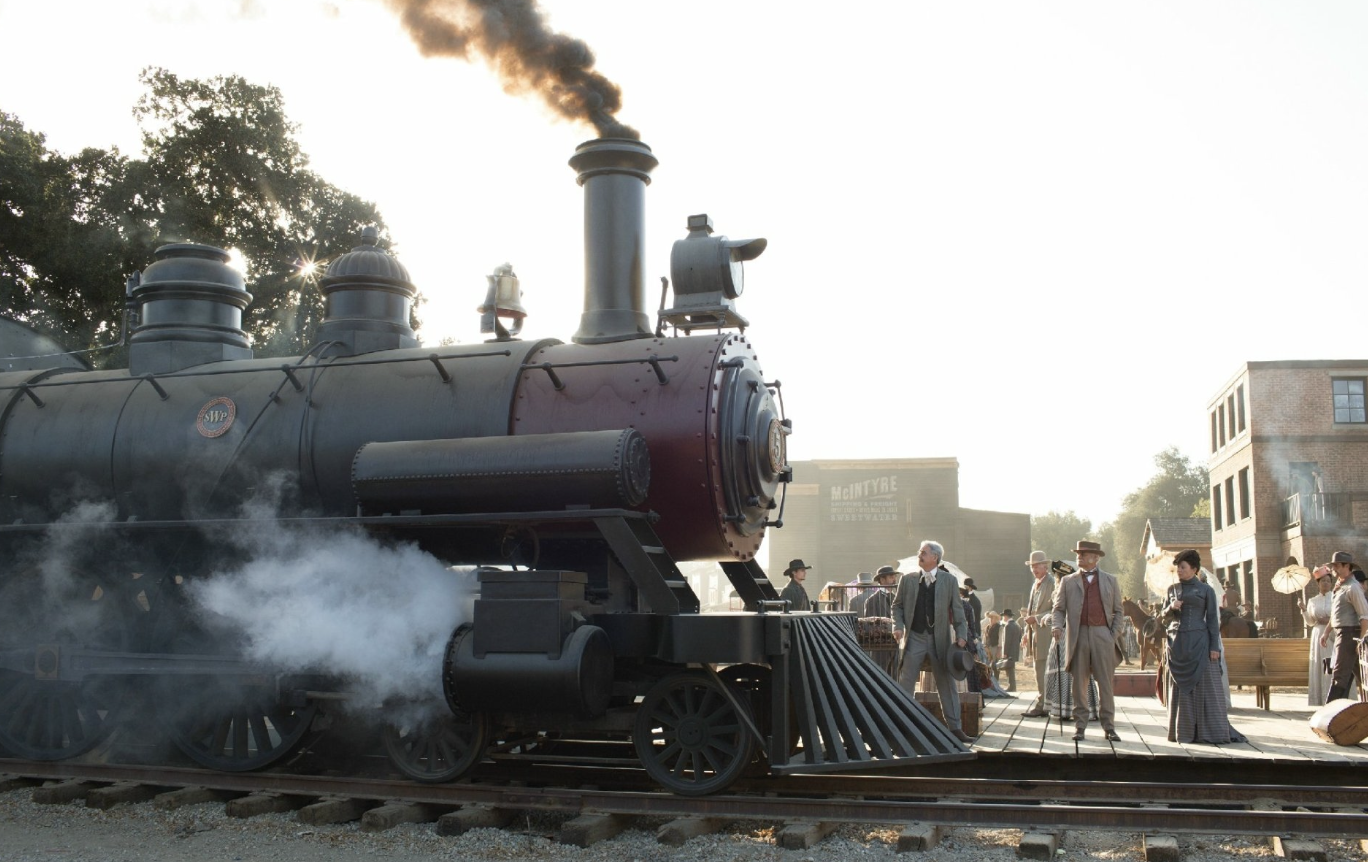
\includegraphics[width=0.8\linewidth]{images/dampflok_fortschritt.png}
\end{center}

\subsection{Die Entwicklung der Eisenbahn in der Schweiz}

Bereits seit den 1820er Jahren entstanden erste Projekte
für ein schweizerisches Eisenbahnnetz.

1847 wurde mit der sogenannten Spanisch-Brödli-Bahn
zwischen Zürich und Baden die erste Eisenbahnlinie eröffnet.

Nach der Gründung des Bundesstaates entwickelte sich
ein stark fragmentiertes Bahnsystem,
in dem private und staatliche Unternehmen miteinander konkurrierten.

Zwischen 1901 und 1909 wurden die grössten Privatbahnen
zu den Schweizerischen Bundesbahnen (SBB) zusammengeführt.

Gleichzeitig entstanden weiterhin regionale Privatbahnen.

Aufgrund fehlender Kohlevorkommen setzte die Schweiz
früh auf die Elektrifizierung des Bahnverkehrs.

Dadurch entwickelte sich die Eisenbahn zu einer zentralen Infrastruktur
des modernen Bundesstaates.

\begin{center}
    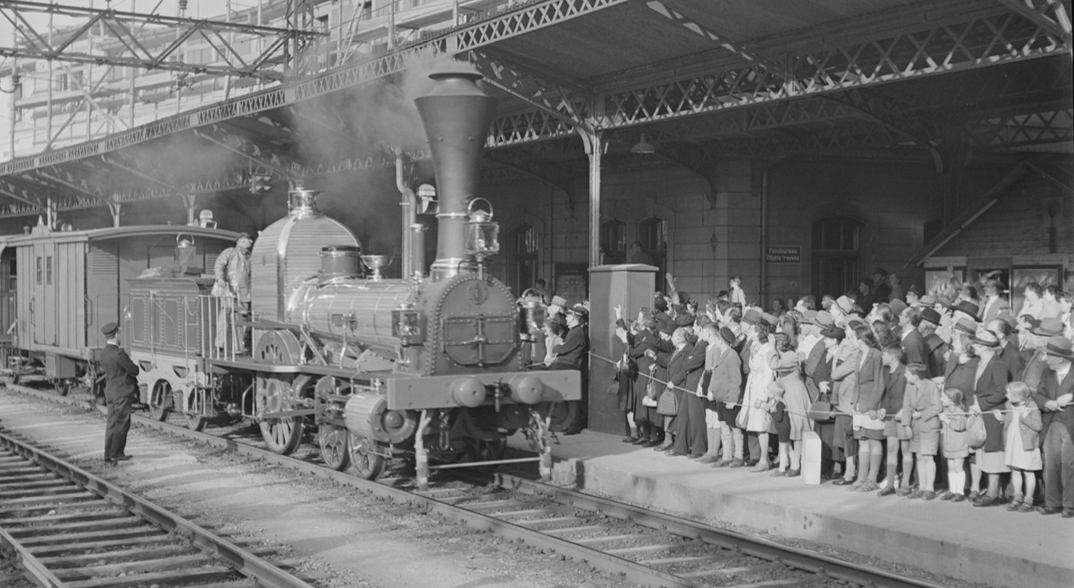
\includegraphics[width=0.8\linewidth]{images/spanisch_broedli_bahn.png}
\end{center}

\subsection{Verkehr, Kommunikation und gesellschaftlicher Wandel}

Die Vorlesung betont,
dass Verkehrssysteme nicht isoliert betrachtet werden können.

Die Entwicklung des Eisenbahnverkehrs
stand in engem Zusammenhang mit neuen Kommunikationsformen.

Dazu gehörten:

\begin{itemize}
    \item die Post
    \item Telegraphennetze
    \item Funktechnik
    \item moderne Sicherungssysteme
\end{itemize}

Transport und Kommunikation entwickelten sich gemeinsam
zu den grundlegenden Infrastrukturen moderner Gesellschaften.

Im Verlauf des 20. Jahrhunderts wandelte sich die Eisenbahn zudem
von einem vorwiegend für Güter genutzten Verkehrsmittel
zu einem Massenverkehrsmittel für die Bevölkerung.

\subsection{Quellenkritik: Das Signalisationssystem der SBB}

Im Zentrum der Quellenanalyse stand das Piktogrammsystem der SBB,
das Ende der 1980er Jahre entwickelt wurde.

Die Quelle besteht aus einer Übersicht der neuen Bahnhofssignalisation
und zeigt standardisierte Symbole für Orientierung,
Dienstleistungen und Verkehrsanschlüsse.

\begin{center}
    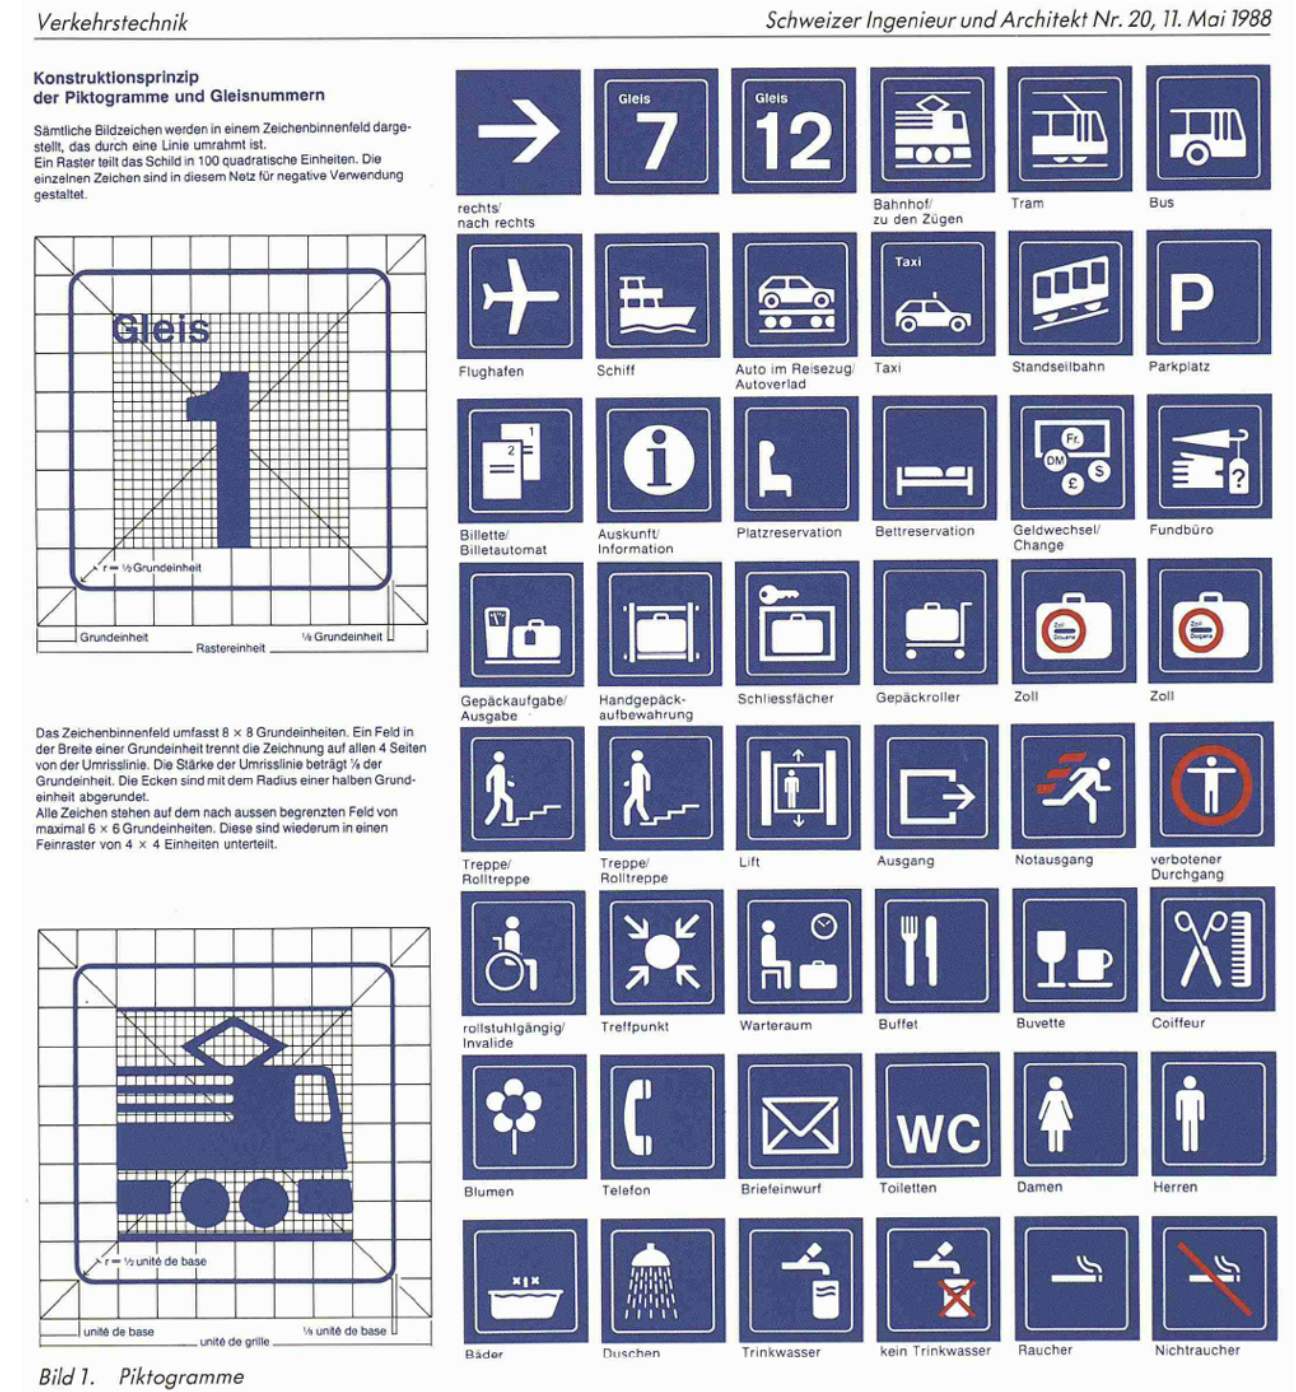
\includegraphics[width=0.9\linewidth]{images/sbb_piktogramme.png}
\end{center}

\paragraph{Äussere Quellenkritik}

Bei der Quelle handelt es sich um eine visuelle Quelle
beziehungsweise um ein technisches Gestaltungskonzept.

Veröffentlicht wurde sie 1988 in der Fachzeitschrift
\textit{Schweizer Ingenieur und Architekt}.

Die Quelle entstand im Umfeld der Schweizerischen Bundesbahnen
und richtet sich sowohl an Fachpersonen
als auch an die breite Öffentlichkeit.

Sie entstand in einer Zeit,
in der die SBB ihre Bahnhöfe modernisierte
und zunehmend auf eine einheitliche Kundenorientierung setzte.

Die Zielgruppe waren nicht mehr nur regelmässige Bahnbenutzer,
sondern auch Gelegenheitsreisende,
Touristen und internationale Fahrgäste.

\paragraph{Innere Quellenkritik}

Die Quelle verfolgt das Ziel,
Orientierung innerhalb komplexer Verkehrsinfrastrukturen
zu vereinfachen.

Die Symbole sollen sprachunabhängig funktionieren
und eine schnelle Informationsaufnahme ermöglichen.

Im Gegensatz zu älteren Beschilderungen
beruht das System auf Standardisierung,
Wiedererkennbarkeit und visueller Klarheit.

Dadurch wird der Bahnhof als übersichtlicher,
effizienter und kundenfreundlicher Raum dargestellt.

Die Gestaltung orientiert sich an internationalen Standards
des Informationsdesigns und der visuellen Kommunikation.

\paragraph{Quelleninterpretation}

Die Quelle zeigt,
dass sich die Rolle der Eisenbahn im Laufe des 20. Jahrhunderts
grundlegend verändert hatte.

Während Bahnhöfe um 1900 vor allem Orte
des Güterverkehrs und des nationalen Reisens waren,
mussten sie in den 1980er Jahren
wachsende Personenströme bewältigen.

Die Signalisation verweist auf neue gesellschaftliche Bedürfnisse:

\begin{itemize}
    \item Mobilität für breite Bevölkerungsschichten
    \item internationale Reisemöglichkeiten
    \item Orientierung unabhängig von Sprache
    \item schnelle Informationsverarbeitung
    \item kundenorientierte Dienstleistungen
\end{itemize}

Die SBB verfolgte mit der neuen Signalisation
das Ziel, Bahnhöfe effizienter nutzbar zu machen
und die Attraktivität des öffentlichen Verkehrs zu steigern.

Die Quelle zeigt somit,
dass technische Infrastruktur zunehmend
auf Benutzerfreundlichkeit und Service ausgerichtet wurde.

Sie kann daher als Ausdruck einer Gesellschaft verstanden werden,
die Mobilität als selbstverständlichen Bestandteil des Alltags betrachtet.

\subsection{Der Taktfahrplan als organisatorische Innovation}

Ein entscheidender Entwicklungsschritt erfolgte 1982
mit der Einführung des schweizweiten Taktfahrplans.

Das Konzept wurde von Samuel Stähli,
Hans Meiner und Jean-Pierre Berthouzoz entwickelt.

Vorbilder fanden sich in den Niederlanden,
bei städtischen Verkehrsbetrieben
und auf einzelnen Bahnstrecken der Schweiz.

Ziel war es,
nicht primär neue Strecken zu bauen,
sondern bestehende Infrastruktur effizienter zu nutzen.

Der Taktfahrplan stellt damit eine organisatorische Innovation dar,
bei der Planung und Koordination wichtiger werden
als technische Neuerungen an Fahrzeugen oder Gleisen.

\subsection{Der „Spinner Club“ und neue Denkweisen}

Die Entwicklung des Taktfahrplans begann bereits Ende der 1960er Jahre.

Eine informelle Arbeitsgruppe innerhalb der SBB,
später als „Spinner Club“ bezeichnet,
arbeitete über Jahre an neuen Konzepten.

Die Gruppe versuchte,
innerhalb einer grossen und stark hierarchischen Organisation
alternative Lösungen für die Zukunft des Bahnverkehrs zu entwickeln.

Die Geschichte des Taktfahrplans zeigt damit,
dass Innovation nicht nur durch neue Technologien entsteht,
sondern auch durch neue organisatorische Ideen.

\begin{center}
    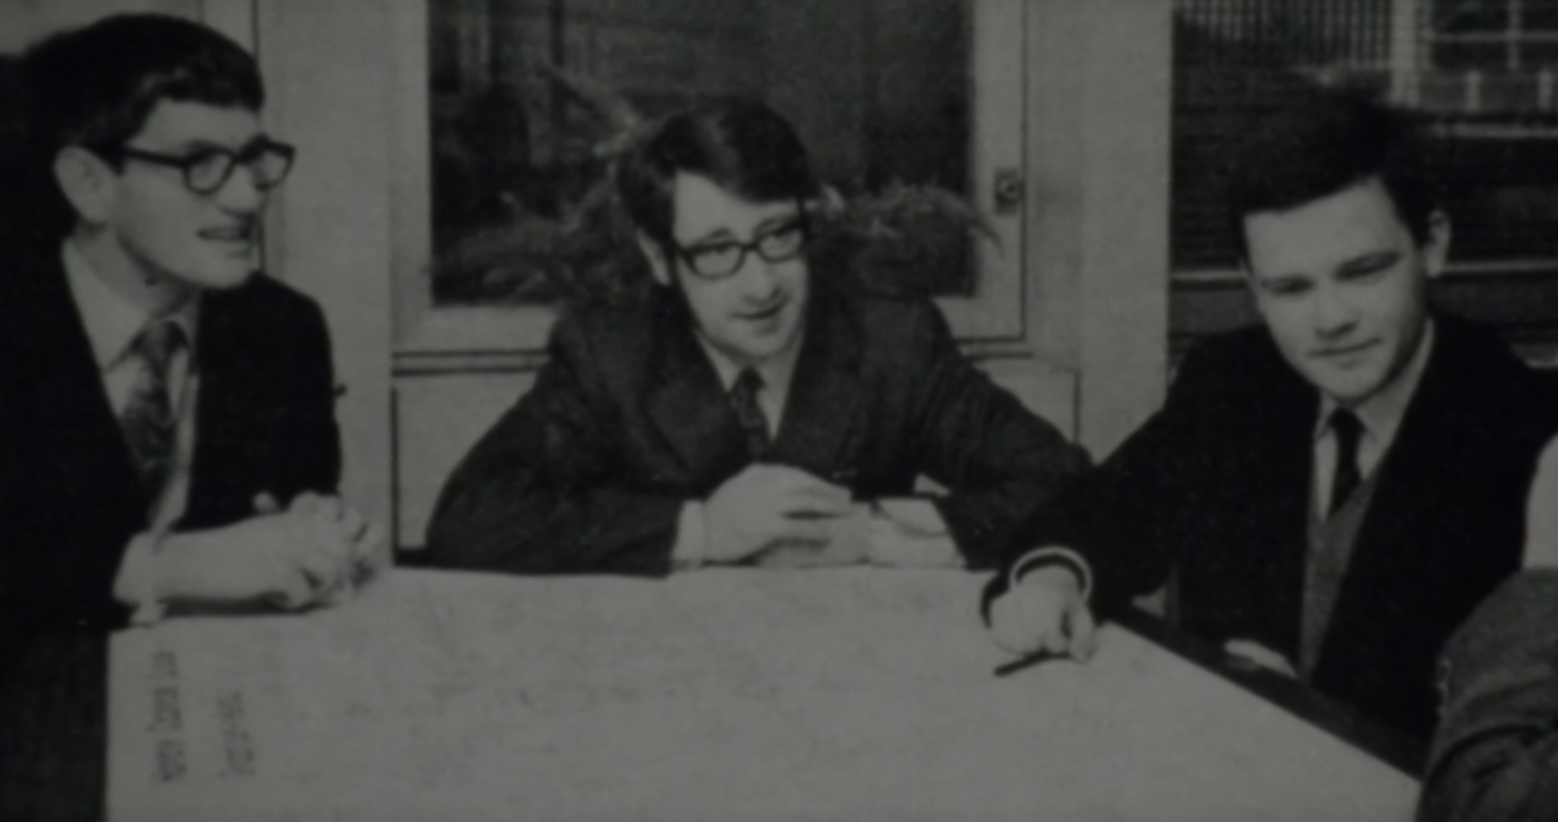
\includegraphics[width=0.7\linewidth]{images/spinner_club.png}
\end{center}

\subsection{Vom Verkehrsmittel zum Mobilitätsangebot}

Mit dem Taktfahrplan veränderte sich die Logik des Bahnbetriebs.

Statt sich ausschliesslich an bestehender Nachfrage zu orientieren,
schufen die SBB ein regelmässiges und leicht verständliches Angebot.

Ziele waren:

\begin{itemize}
    \item Effizienzsteigerung
    \item bessere Anschlüsse
    \item höhere Attraktivität des Bahnverkehrs
    \item Konkurrenzfähigkeit gegenüber dem Auto
\end{itemize}

Die Eisenbahn entwickelte sich dadurch
von einem reinen Transportmittel
zu einem umfassenden Mobilitätssystem.

\begin{center}
    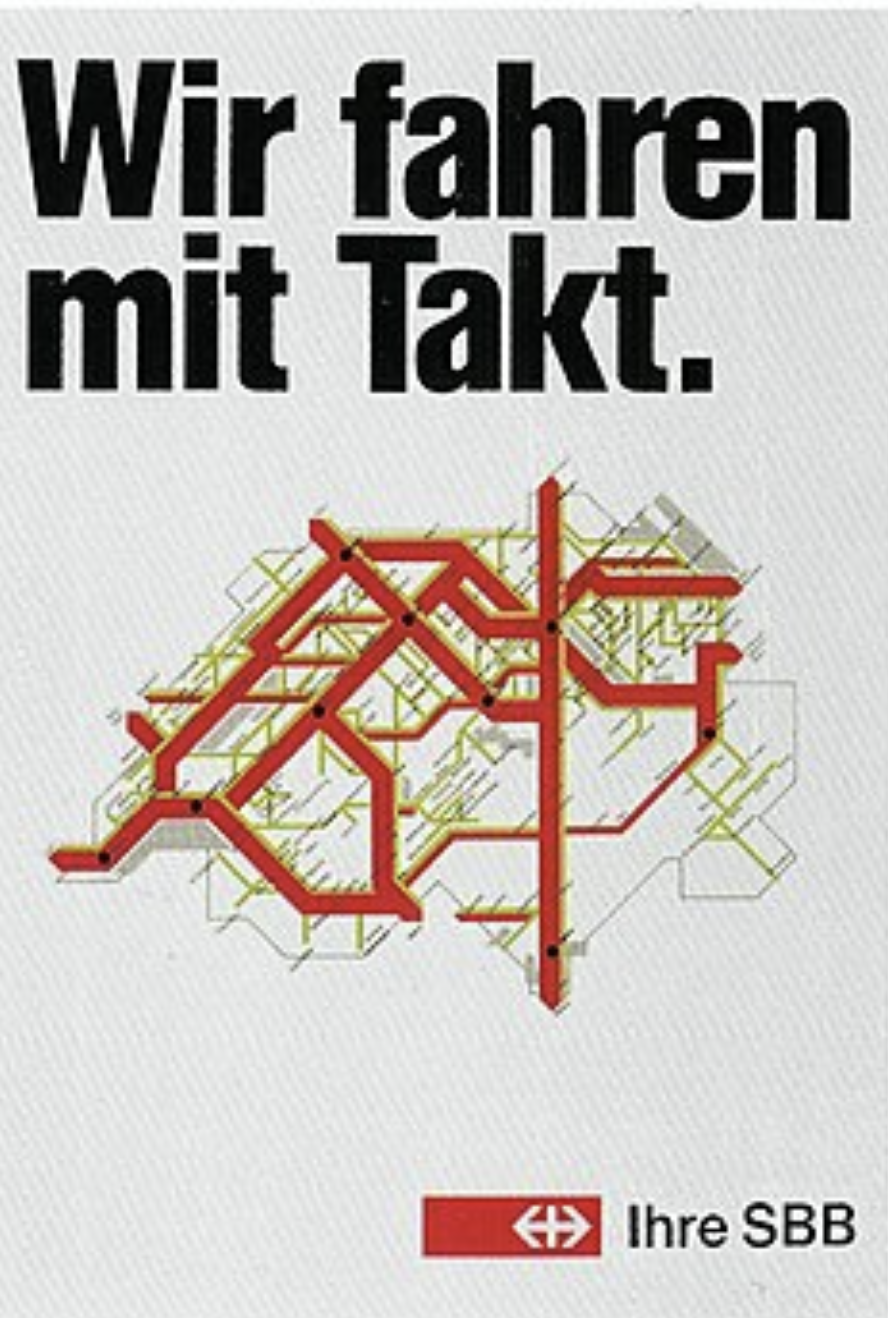
\includegraphics[width=0.55\linewidth]{images/wir_fahren_mit_takt.png}
\end{center}

\subsection{Zentrale Erkenntnisse}

Die Geschichte der Eisenbahn zeigt,
dass technische Innovationen stets mit organisatorischen
und gesellschaftlichen Veränderungen verbunden sind.

Die Vorlesung verdeutlicht insbesondere:

\begin{itemize}
    \item die Rolle der Eisenbahn für die Industrialisierung
    \item die Entstehung nationaler Infrastrukturen
    \item die Bedeutung von Kommunikation und Verkehr
    \item den Wandel zu kundenorientierten Verkehrssystemen
    \item die Bedeutung organisatorischer Innovationen wie des Taktfahrplans
\end{itemize}

Die zentrale These lautet:

Die Entwicklung der Eisenbahn ist nicht nur eine Geschichte
technischer Maschinen und Fahrzeuge.
Sie ist zugleich die Geschichte einer Gesellschaft,
die Mobilität, Orientierung und Vernetzung
zu zentralen Bestandteilen ihres Alltags macht.